%!TEX root = main.tex
  
% levels: entity -- semantic -- syntactic
% careful about elems and Gamma concatenation as primitive constructor menas trees. Better to do finit maps or sequences
% Why need new entdecls from sig extraction?
% {}^\theta{}F({}^\varphi M) \leadsto (M, \varphi) direct mode result, compilation mode

% type classes support recursive instances, why is this possible?
\chapter{Elaboration Semantics}\label{ch:homods}
 
In a first-order module system, functor application can propagate types in the parameter to the functor result. True higher-order semantics is useful for compilation of efficient module code \cite{shao98}. More importantly, type propagation is necessary to make some sound programs typecheck. THO semantics also reflects the dependent type structure of functors. Types in the functor parameter may also be generative, as in the case of datatypes and types in opaquely ascribed substructures. These generative types have to be faithfully propagated during functor application. Functors complicate type propagation because types in the functor result may be computed from multiple sources. As in the first-order case, types may be locally defined in the result or propagated from the parameter. Applications of formal functors (\ie, functors in the functor parameter) in the functor result should also propagates types. Collectively, generation of fresh instances of generative types and formal functor applications are called \emph{functor actions}, which must be performed during elaboration of functor application to maximize type propagation.    
 
As in other accounts of module system designs, I present the THO module system as an elaboration semantics. The syntactic module language is elaborated to a semantic representation. Unlike prior accounts, this semantics will use an entity calculus that captures the functor actions in a program. The entity calculus is a third level of representation distinct from the syntactic and semantic representations. It assumes that each type is given a unique name, an entity variable. Unlike other internal languages, the entity calculus only plays a role in elaboration. Entity calculus terms are translated to IL types by the time code reaches the optimization stages of a compiler. 
      
Elaboration accomplishes the following:
\begin{enumerate}   
	\item Produces a static environment mapping variables to static descriptions of values, types, structures, functors, and signatures
	\item Produces a typed abstract syntax
	\item Produces entity expressions used in representing functor actions
	\item Typechecks the program
\end{enumerate}

For simplicity, the discussion of (2) will be postponed to chapter~\ref{ch:translation}. Fig.~\ref{fig:overview} shows the major components of the elaboration process and how they are related. 

\begin{figure}
\begin{center}
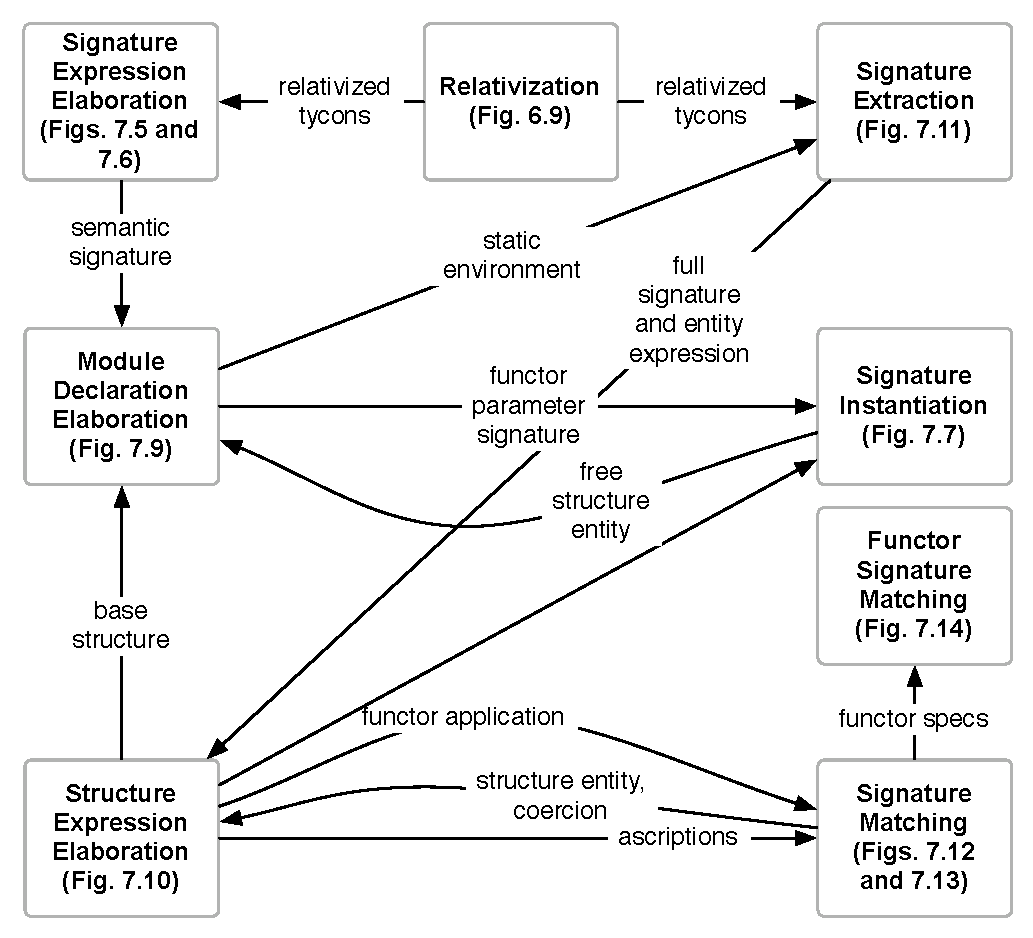
\includegraphics[scale=0.8]{figs/overview}
\end{center}
\caption{Map of elaboration processes}
\label{fig:overview}
\end{figure}
 
% \section{Why Higher-Order Functors?}
% The Fox project at CMU demonstrated that functors are valuable for the design and organization of extensible software systems. Shao~\cite{shao:parameterizedsigsandho}  demonstrates that higher-order functors are necessary for precisely expressing the import signature of a module that refers to externally defined functors. This idea is motivated by the \emph{fully functorized style} originally espoused by Tofte. 


\section{Elaboration Representations}
Elaboration is mainly concerned with the construction of a static environment. Secondarily, the elaborator produces typed abstract syntax, an entity environment, and an entity expression. The static environment contains the visible static information in the elaborated program. The static information comes in the form of semantic representations of signatures and type information. 

\begin{lstlisting}
sig
   type t [$\rho_t$] 
   type u = int 
   structure M [$\rho_M$] : sig type s [$\rho_s$] end
end
\end{lstlisting}
 
The entity environment contains static information that may have been occulted by shadowing and the functor actions describing the production of new static information during functor application. Much of elaboration is concerned with constructing the correct entity environment and using them to interpret entity paths. 

\section{Semantic Objects}
%!TEX root = ../main.tex
\begin{figure}
	\hrule
\[\begin{array}{rcll}
       s^p & ::= &  arity~|~\Sigma~|~\Sigma^f& \textrm{primary spec}\\
       \Sigma & ::= & \emptyset_{sig}~|~[x\mapsto (\rho,
       s^p)]\Sigma & \textrm{semantic signature}\\
       & ~~| & [x\mapsto \mathbb{C}^\lambda]\Sigma~|~[x\mapsto
       \mathbb{T}]\Sigma \\ 
	M & ::= & (\Sigma, R) & \textrm{full signature}\\
        \Sigma^f & ::= & \Pi\rho:\Sigma.\Sigma & \textrm{functor signature}\\
	F & ::= & (\Sigma^f, \psi) & \textrm{full functor signature}\\
        \gamma & ::= &
        \mathfrak{T}~|~\mathfrak{C}^\lambda~|~\Sigma~|~\Sigma^f & \textrm{static binding}\\
        & ~~| & (\rho, M)~|~(\rho,
        F) \\
	\Gamma & ::= & \emptyset_{se}~|~\Gamma[x\mapsto \gamma] &
        \textrm{static type environment}\\
\end{array}\]
The static bindings for structures and functors include the entity
variable to permit direct construction of entity paths during
signature extraction, structure path, and functor path elaboration.  
\hrule
\caption{Semantic representations}
\label{fig:semanticobjs}
\end{figure}
A semantic signature is a sequence of signature elements, symbol to spec bindings. Signature elements can be volatile ($s^p$), definitional ($\mathbb{C}^\lambda$), or a value spec ($\mathbb{T}$). Note that all signature spec elements must be relativized. Nonvolatile elements including definitional tycons $\mathbb{C}^\lambda$ and value specs $\mathbb{T}$ need only specify their fixed static description. Volatile primary specs ($s^p$) such open ones $arity$, structures $\Sigma$, and functors $\Sigma^f$ may be instantiated by signature matching and thus must have a corresponding binding in the entity environment indexed by entity variables. A \emph{full signature M} gives a full semantic description of a structure. It is comprised of a semantic signature $\Sigma$ and a structure entity $R$ that interprets all the open specifications in $\Sigma$. 

A semantic functor signature $\Sigma^f$ binds an entity variable for the functor parameter $\rho$ in the functor result signature. A full functor signature $F$ is comprised a semantic functor signature $\Sigma^f$ and a functor entity $\psi$ that when evaluated will interpret all the open specifications in the functor result signature. 

$\gamma$ is a static binding, to which the static environment $\Gamma$ maps identifiers. For value identifiers, the static description is a semantic type expression $\mathfrak{T}$. For tycon definitions, the static description is $\mathfrak{C}^\lambda$. There is no static binding for open tycon because all tycons are either defined or instantiated in the static environment.  For signature and functor signature identifiers, the static descriptions are semantic signatures ($\Sigma$) and semantic functor signature ($\Sigma^f$). For structure and functor identifiers, the static descriptions are full signatures and full functor signatures respectively. Some static binding (namely for structures and functors) consist of the full signature or full functor signature coupled with the entity variable for that structure or functor. The entity variable is used to construct entity paths during signature extraction and elaboration. 

Tycons in signatures and in static environments differ in that tycons
in the former will have been relativized during signature elaboration
or extraction. Unlike static environments that may be extended
throughout the elaboration process, signatures do not change. Hence to
ensure that volatile tycons in signatures have an appropriate
interpretation, they must be relativized with respect to the entity
environment. 

\begin{figure}
\begin{center}
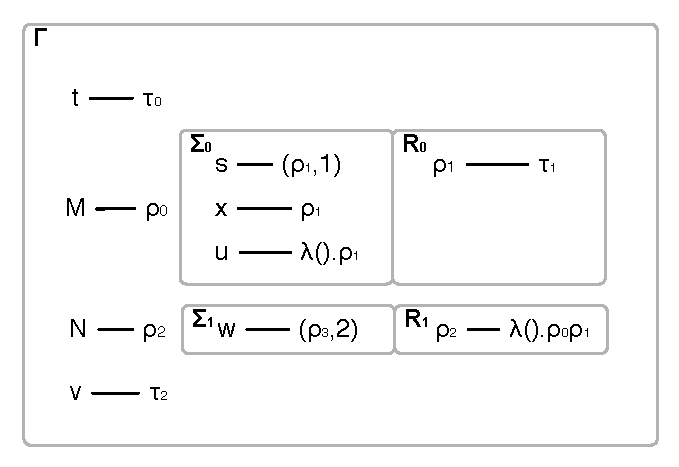
\includegraphics{figs/fig-staticenv-sigs}
\end{center}
\caption{Schematic of static environment}
\label{fig:staticenv-sigs}
\end{figure}

In Fig.~\ref{fig:staticenv-sigs}, the static environment depicted
exhibits the heterogeneous form of the definition. The first layer
contains semantic tycons, those types directly bound by the static
environment. The second layer consist of the tycons $s, u,$ and $w$ bound in semantic
signatures $\Sigma_0$ and $\Sigma_1$ embedded inside of the static
environment. These semantic signatures contain relativized tycons. The
full signature for structures also include the structure entity
expressions $R_0$ and $R_1$ which define the instantiation of the open
tycons in the corresponding semantic signature.  


\section{Notation}\label{sec:elabnotation}

If $p$ is a symbolic path and $\Sigma$ is a semantic signature, then $p\in\Sigma$ means that following $p$ in $\Sigma$ reaches a spec. If $p$ is a singleton, then $\Sigma$ must contain a binding $p\mapsto spec$. Otherwise, if $p$ is nonsingleton, then $p=xp'$ such that $x$ is a symbol and $p'$ is a symbolic path such that $\Sigma$ contains a binding $x\mapsto (\rho,\Sigma')$ and $p'\in\Sigma$. 

$\Sigma(p)$ is the spec reached by following $p$ in $\Sigma$. The notation $\EP(\Sigma,p)$ denotes the entity path associated with the signature spec referred to by symbolic path $p$. The entity path is comprised of the entity variables on the path to the element. For example, if the signature is $\Sigma = [A\mapsto(\rho_A,[B\mapsto (\rho_B, [t \mapsto (\rho_t, 0)])])]$, then $\Sigma_{ep}(A.B.t) = \rho_A\rho_B\rho_t$. The same notation is extended to static environments. 

Static environment lookup is expressed as $\Gamma(p)$ where $p$ is the symbolic path to the static binding. If $p$ is a singleton, then the static environment lookup would simply return the corresponding static binding. As will be demonstrated below, static environment lookup sometimes requires an entity environment lookup. This is the case when the component being looked up is a definitional tycon in a nonsingleton path. Depending on what kind of entity $p$ refers to, the lookup is handled differently:
\begin{description}
\item[tycon]
\begin{description}
\item[singleton path $p=x$] The semantic tycon is $\Gamma(x)$.
\item[nonsingleton $p=q.x$] $\Gamma(q)$ produces a full signature ($\Sigma_q,R_q$). Let $\Upsilon_q = \Upsilon^{clo}\Upsilon^{lcl}$ where $R_q = \langle \Upsilon^{lcl}, \Upsilon^{clo}\rangle$. 

If $\Sigma_q(x) = (\rho_x,n)$, then $\Gamma(p) = \Upsilon_q(\rho_x)$. 

If $\Sigma_q(x) = \mathbb{C}^\lambda$, then $\Gamma(p) = $ the interpretation of $\mathbb{C}^\lambda$ under $\Upsilon_q$. 

Note that all tycons are interpreted using the structure entity closest to the occurrence. 
\end{description}
\item[full signature or a full functor signature] $\Gamma(p)$ denotes a pair $(\vec{\rho}, M)$ such that $\vec{\rho}$ is the entity path to the structure static binding and $M$ is the full signature of that structure. For example, for $\Gamma=[A\mapsto(\rho_A,([B\mapsto(\rho_B, \Sigma_B)], R_A))]$, $\Gamma(A.B) = (\rho_A\rho_B, (\Sigma_B,R_A(\rho_A\rho_B)))$. 
\end{description}

\section{Elaboration Modes}
During elaboration, entity expressions are both produced and consumed to aid in typechecking. Elaboration occurs in two simultaneous modes: the \emph{direct mode} and the \emph{entity compilation mode}. Direct mode consists of core language type checking, direct construction of entity expressions (such as tycon declaration elaboration and signature instantiation), and evaluation of entity expressions from the static information uncovered during elaboration. The main results of this mode are a static environment mapping symbolic names to static descriptions and an entity environment mapping entity variables to entities. The evaluation of entity expressions may produce new entities which added to static and entity environments. The entity compilation mode compiles functor actions into entity expressions.   

Elaboration is entirely a compile-time process. The entity language is distinct from core and module languages. The language is parallel to the semantic representation and the syntactic language. Elaboration translates core and module languages to typed abstract syntax and entity expressions. The part of elaboration that produces entity expressions and declaration is called \emph{static entity compilation}. Because the entity language is intended to describe functor actions, which are not encoded in the typed abstract syntax, the two are complementary. When the elaborator reaches a functor application in the source, the corresponding application entity expression must be evaluated to produce the static information for the result. Entity expression evaluation yields structure entities. 
   
\section{Entity Compilation Mode}
Besides the direct elaboration mode for the evaluation of entity expressions, described in chapter~\ref{ch:entitycalc}, the elaborator must have an entity compilation mode that produces the entity expressions and semantic representations of the modules from the syntax. The process of the compilation mode is the bulk of the elaboration semantics. Entity expressions for both structures and functors are compiled from the raw implicitly typed abstract syntax trees and the contextual environments used during elaboration. The compilation mode elaboration is the subject of the remainder of this chapter. 

The compilation mode elaboration compiles abstract
syntax trees to entity expressions. All of elaboration takes place
under a static environment $\Gamma$. Recall that semantic
signatures pair all static primary components with entity variables
and replace all occurrences of such primaries with a canonical entity path to the corresponding static entity in the entity environment, which is calculated by relativization. Values are classified by their type. Structures are described by their full signature consisting of a structure entity and a signature. A functor static description is a full functor signature, comprised of a functor entity expression (\ie, a $\lambda$-expression) and a functor signature. The main elaboration judgments are the following:\\[-5mm]
 
\begin{tabular}{ll}
        $\Gamma,\Upsilon,\Sigma\vdash C^s \Rightarrow_{mt} \mathfrak{C}^s$ & monotype elaboration\\
        $\Gamma,\Upsilon,\Sigma\vdash C^\lambda \Rightarrow_{tyc} \mathfrak{C}^\lambda$ & tycon elaboration\\
        $\Gamma,\Upsilon,\Sigma\vdash T \Rightarrow_{te} \mathfrak{T}$ & type elaboration\\
\end{tabular}\\

The above judgments produce semantic monotypes/tycons/type expressions from syntactic ones. Tycon elaboration's sole role is during elaboration of tycon declarations (rule~\ref{eq:typedefdecl}). \\[-5mm]

\begin{tabular}{ll}       
        $\Upsilon\vdash \mathfrak{C}^s \searrow^{mt} \mathbb{C}^s$ & monotype relativization\\
        $\Upsilon,\Sigma\vdash \mathfrak{C}^\lambda \searrow^{tyc} \mathbb{C}^\lambda$ & tycon relativization\\
        $\Upsilon,\Sigma\vdash T \searrow^{te} \mathbb{T}$ & type expression relativization
\end{tabular}\\

The relativization judgment produce relativized tycons from syntactic ones. The entity environment $\Upsilon$ is used to relativize the nonlocally defined tycons. The signature $\Sigma$ is used to construct relativized entity paths for locally defined tycons. Signature extraction and elaboration rely on relativization. \\[-5mm]

\begin{tabular}{ll}      
        $\Gamma,\Upsilon,\Sigma\vdash sigexp \Rightarrow_{sig} \Sigma'$ & signature elaboration\\
        $\Gamma,\Upsilon,\Sigma\vdash fsgexp \Rightarrow_{fsg} \Sigma^f$ & functor signature elaboration\\
        $\Upsilon^{clo},\Upsilon^{lcl}\vdash \Sigma \uparrow \Upsilon^{lcl}$ & signature instantiation\\
        $\Gamma,\Upsilon\vdash d^m \Rightarrow_{decl} (\eta,\Gamma',\Upsilon')$ & module declaration elaboration\\
        $\Gamma,\Upsilon\vdash strexp \Rightarrow_{str} (M, \varphi)$ & structure expression elaboration\\
        $\Upsilon\vdash\Gamma\hookrightarrow \Sigma$ & signature extraction\\
        $\Upsilon\vdash(M,\varphi):\Sigma\Rightarrow_{match} (M_c,\varphi_c)$ & signature matching\\
        $\Upsilon\vdash F \preceq \Sigma^f \Rightarrow_{fsgmtch} (\psi_c, \theta_c)$ & functor signature matching
\end{tabular}

\section{Type Constructors}
The syntactic type language is a subset of the semantic tycon language. Before proceeding, the elaborator must first elaborate the syntactic types to semantic tycons. The elaboration is simply a syntax-directed recursive translation. 

The syntactic type language elaborates to the semantic type language. Elaboration interprets the symbolic paths in tycon application $p(\vv{C^s})$ and evaluates the application by standard $\beta$-reduction. Note that tycon elaboration $\Rightarrow_{tyc }$ elaborates and therefore reduces under $\lambda$-abstraction. This ensures that tycon definitions are fully reduced. Because $\lambda$s cannot be nested, this reduction is well-defined and normalizing. The normal form is defined as $\mathfrak{C}^{nf}$ in fig.~\ref{fig:semtypesystem}. 

\begin{figure}
\centering
\fixedCodeFrame{
\small
\setlength{\tabcolsep}{0ex}
\renewcommand{\arraystretch}{1.1}
~\\[2mm]
\fbox{$\Gamma,\Sigma\vdash C^s \Rightarrow_{mt} \mathfrak{C}^s$}

\begin{equation}
\Gamma,\Sigma\vdash \alpha \Rightarrow_{mt} \alpha
\label{eq:alpha}
\end{equation}

\begin{equation}
\infer{\Gamma,\Sigma\vdash p(\vv{C^s}) \Rightarrow_{mt}
 \mathfrak{C}^s_a}
{\begin{array}{c}
\Gamma,\Sigma\vdash C^s_i \Rightarrow_{mt} \mathfrak{C}^s_i~\forall i\in[1,|\vv{C^s}|]\\
(\mathsf{entpath}(\Gamma,\Sigma,p))(\vv{\mathfrak{C}^s}) \Downarrow_{tyc} \mathfrak{C}^s_a
\end{array}}
\label{eq:tycapp}
\end{equation}

\fbox{$\Gamma,\Sigma\vdash C^\lambda 
\Rightarrow_{tyc} \mathfrak{C}^\lambda$}

\begin{equation}
\infer{\Gamma,\Sigma\vdash \lambda\vec{\alpha}.C^s
  \Rightarrow_{tyc}\lambda\vec{\alpha}.\mathfrak{C}^s}
  {\Gamma,\Sigma\vdash C^s \Rightarrow_{mt} \mathfrak{C}^s}
% This rule is necessary to permit relativization of type definitions
% that area always enclosed by a single lambda. 
\end{equation}

\fbox{$\Gamma,\Sigma\vdash T \Rightarrow_{te} \mathfrak{T}$}

\begin{equation}
\infer{\Gamma, \Sigma\vdash \mathsf{typ}(C^s) 
\Rightarrow_{te} \mathsf{typ}(\mathfrak{C}^s)}
{\Gamma, \Sigma\vdash C^s \Rightarrow_{mt} \mathfrak{C}^s}
\end{equation}

\begin{equation}
\infer{\Gamma, \Sigma\vdash \forall\vec{\alpha}.C^s \Rightarrow_{te}
  \forall\vec{\alpha}.\mathfrak{C}^s}
{\Gamma, \Sigma\vdash C^s \Rightarrow_{mt} \mathfrak{C}^s}
\end{equation}

\begin{equation*}
\mathsf{entpath}(\Gamma,\Sigma,p) = \left\{ \begin{array}{ll}
\mathsf{EP}(\Sigma,p)& \textrm{if }p\in\Sigma\\
 \Gamma_{ep}(p) & \textrm{o.w.}
\end{array}
\right. 
\end{equation*}
}
\caption{Monotype and tycon elaboration}
\label{fig:tyconelab}
\end{figure} 

Note that the tycon may be occuring inside a signature spec, in which case it may refer to entity paths for preceding specs. 

\begin{lstlisting}
sig 
  type t
  type u = t
end
\end{lstlisting}

During the elaboration of the above, t will be given an entity variable. When elaborating the occurrence of tycon t in the definition of u, t is not the static environment. It can only be found in the partial semantic signature produced by elaborating the open spec for t. Signature specs may contain relativized tycons, entity paths,
referencing entities declared earlier in the same semantic signature. These preceding signature specs (forming a semantic signature $\Sigma$ itself)
help construct an entity path for symbolic paths not defined in the
static environment. Rule~\ref{eq:tycapp} uses $\entpath$ to calculate the entity path using static and entity environments. In order
to fully relativize such a symbolic path, the $\entpath$ metafunction
needs to first lookup the symbolic path in the preceding signature
specs $\Sigma$, which contains all the preceding specs in the current signature and only if that fails does it look up in the static environment.  


The type elaboration judgments preserve the well-kinding defined in chapter~\ref{ch:typesystem}.

\begin{lemma}[Monotype Elaboration Preserves Kinding]
If $\Gamma,\emptyset_{knds}\vdash C^s : \Omega$ and $\Gamma,\Upsilon\vdash C^s \Rightarrow_{mt} \mathfrak{C}^s$, then $\emptyset_{knds}\vdash \mathfrak{C}^s : \Omega$. 
\end{lemma}

\begin{lemma}[Tycon Elaboration Preserves Kinding]
If $\Gamma,\emptyset_{knds}\vdash C^\lambda : \Omega^n \Rightarrow
\Omega$ and $\Gamma,\Upsilon\vdash C^\lambda \Rightarrow_{tyc}
\mathfrak{C}^\lambda$, then $\emptyset_{knds}\vdash \mathfrak{C}^\lambda : \Omega^n \Rightarrow \Omega$.
\end{lemma}

\section{Signature Elaboration}
The role of signature elaboration is to relativize tycons, to reduce where type clauses to type definitions, and to decorate all specs corresponding to static entities with  entity variables. The elaboration judgment uses static and entity environment to interpret symbolic paths in tycon definitions. However, not all symbolic paths are bound in the static environment. For example, in the following signature, the type definition for u mentions tycon t which does not have a corresponding structure entity at this point, hence tycon t will not be in static and entity environment. 

\begin{lstlisting}
sig type t type u = t end
\end{lstlisting}

Rule~\ref{eq:specs} composes the result of elaborating the individual specs. Elaborating subsequent specs in the same signature will require a context (a signature) that includes all the previously elaborated specs $\Sigma$ and the newly elaborated spec $\Sigma'$.  

%!TEX root = ../principles.tex
\begin{figure}
\centering
\fixedCodeFrame{
\small
\setlength{\tabcolsep}{0ex}
\renewcommand{\arraystretch}{1.1}
~\\[2mm]
\fbox{$\Gamma,\Upsilon,\Sigma\vdash sigexp \Rightarrow_{sig} \Sigma'$}
	
\begin{equation}
\infer{\Gamma,\Upsilon,\Sigma\vdash x \Rightarrow_{sig} \Gamma(x)}
{\strut} 
\label{eq:emptysig}
\end{equation}

\begin{equation}
\infer{\Gamma,\Upsilon,\Sigma\vdash sigexp~\textbf{where type}~p = C^\lambda\Rightarrow_{sig}\mathsf{rebind}(p,\mathbb{C}^\lambda,\Sigma')}
	{\begin{array}{c}
	  \Gamma,\Upsilon,\Sigma\vdash sigexp\Rightarrow_{sig}\Sigma'\qquad
	  \Sigma'(p) = (\rho,n)\\ \Gamma,\Upsilon\vdash C^\lambda \Rightarrow_{tyc} \mathfrak{C}^\lambda\qquad 
          \Gamma,\Upsilon,\Sigma\Sigma'\vdash C^\lambda \searrow^{tyc} \mathfrak{C}^\lambda \\
          \Upsilon\vdash \mathfrak{C}^\lambda \searrow^{tyc} 
          \mathbb{C}^\lambda\qquad |\mathbb{C}^\lambda|=n
	 \end{array}} 
\label{eq:wheretype}
\end{equation}

\begin{equation}
\infer{\Gamma,\Upsilon,\Sigma\vdash \textbf{sig } specs \textbf{ end} \Rightarrow_{sig} \Sigma'}
	{\begin{array}{c}
	\Gamma,\Upsilon,\Sigma\vdash specs \Rightarrow_{specs} \Sigma'
	\end{array}} 
\label{eq:sigspecs}
\end{equation}

$\mathsf{rebind}(p,\mathbb{C}^\lambda,\Sigma)$ replaces the
binding $[x\mapsto (\rho,n)]$ in $\Sigma$ with $[x \mapsto 
\mathbb{C}^\lambda]$ where $p$ ends in $x$. 

\fbox{$\Gamma,\Upsilon,\Sigma\vdash specs \Rightarrow_{specs} \Sigma$}
\begin{equation}
\infer{\Gamma,\Upsilon,\Sigma\vdash \emptyset_{specs} \Rightarrow_{specs} \emptyset_{sig}}
{\strut}
\end{equation}

\begin{equation}
\infer{\Gamma,\Upsilon,\Sigma\vdash spec,specs \Rightarrow_{specs} \Sigma'\Sigma''}
{\Gamma,\Upsilon,\Sigma\vdash spec \Rightarrow_{spec} \Sigma' \qquad \Gamma,\Upsilon,\Sigma\Sigma'\vdash specs \Rightarrow_{specs} \Sigma''}
\label{eq:specs}
\end{equation}

}
\caption{Signature elaboration}
\label{fig:elabsig}
\end{figure}

\begin{figure}
	\centering
	\fixedCodeFrame{
	\small
	~\\[2mm]
	\fbox{$\Gamma, \Upsilon, \Sigma \vdash spec \Rightarrow_{spec} \Sigma'$}
\begin{equation}
\infer{\Gamma,\Upsilon,\Sigma\vdash\textbf{type
                  }\vec{\alpha}~t\Rightarrow_{spec} [t\mapsto (\rho,|\vec{\alpha}|)]}
{(\rho\textrm{ fresh in }\Gamma\textrm{ and
                  }\Upsilon)} 
\end{equation}
% Do we need to extend the static environment during elaboration of
% the subsequent specs? The only reason we might need to is to support
% relativization. I think we have to. 
\begin{equation}
\infer{\Gamma,\Upsilon,\Sigma\vdash\textbf{type }t=C^\lambda\Rightarrow_{spec} [t\mapsto \mathbb{C}^\lambda]}
{\Gamma,\Upsilon\vdash C^\lambda \Rightarrow_{tyc} \mathfrak{C}^\lambda\qquad \Upsilon,\Sigma\vdash \mathfrak{C}^\lambda \searrow^{tyc}
 \mathbb{C}^\lambda}
\label{eq:typedefspec}
\end{equation}

\begin{equation}
              \infer{\Gamma,\Upsilon,\Sigma\vdash\textbf{val }x:T
                 \Rightarrow_{spec} [x\mapsto\mathbb{T}]}
{\Gamma,\Upsilon\vdash T \Rightarrow_{te} \mathfrak{T}\qquad \Upsilon,\Sigma\vdash \mathfrak{T} \searrow^{tyc} \mathbb{T}}
\label{eq:valspec}
\end{equation}

\begin{equation}
\infer{\begin{array}{c}
    \Gamma,\Upsilon,\Sigma\vdash\textbf{structure }x :
                  sigexp
                  \Rightarrow_{spec} [x\mapsto
                  (\rho,\Sigma')]
\end{array}}
		{\begin{array}{c}
                    \Gamma,\Upsilon,\Sigma\vdash sigexp
                    \Rightarrow_{sig}
                    \Sigma'\qquad
                    (\rho~\textrm{fresh in }\Gamma\textrm{ and
                    }\Upsilon) 
              \end{array}}
\end{equation}

\begin{equation}
\infer{\begin{array}{c}
\Gamma,\Upsilon,\Sigma\vdash\textbf{functor }f(X: sigexp_1):sigexp_2\\
   \Rightarrow_{spec} [f\mapsto(\rho,\Pi\rho_x:\Sigma_1.\Sigma_2)]
\end{array}}
		{\begin{array}{c}
\Gamma,\Upsilon,\Sigma\vdash sigexp_1 \Rightarrow_{sig}
\Sigma_1 \qquad
(\rho_x\textrm{ and }\rho~\textrm{fresh in }\Gamma\textrm{ and }\Upsilon )\\
\Gamma,\Upsilon,\Sigma[X\mapsto(\rho_x,\Sigma_1)]\vdash
sigexp_2 \Rightarrow_{sig} \Sigma_2\\
% \qquad \psi=\langle\lambda\rho_x.\Sigma_2 ;
%  \Upsilon\rangle % [4/8/10] Is this the correct closure environment? Can \Sigma_2 mention local entities? Yes, but those are local, therefore, they should be interpreted locally and not by the closure, which only interpret nonlocal entities.  
\end{array}}
\label{eq:fctspec}
\end{equation}

	}
	\caption{Signature spec elaboration}
	\label{fig:elabspec}
\end{figure}   

Signature spec elaboration produces entity variables for each static
component (\emph{i.e.}, open type specs, structure spec, and functor
spec) and puts them in the resultant semantic
signature. Rules~\ref{eq:typedefspec} and~\ref{eq:valspec} relativize
semantic tycons and type expressions respectively. 

In particular, the signature $\Sigma$ is needed when relativizing specs in a signature $\Sigma'$ that contain symbolic paths defined within the same $\Sigma$. Latter specs can contain symbolic paths declared in earlier specs within the same signature. Because the signature is not yet fully elaborated and does not correspond to any full signature, it is neither defined in the static environment nor the entity environment, each of which only mapping paths defined outside of the signature currently being elaborated. 


Rule~\ref{eq:fctspec} elaborate the formal parameter signature $sigexp_1$ and then the functor body signature $sigexp_2$ with the signature context extended with a spec corresponding to the formal parameter. 

Let $AT(\cdot)$ denote the set of all atomic tycons ($\tau^n$) in $\cdot$. 
The following lemma guarantees that all tycons are fully relativized by the relativization judgment. 

\begin{lemma}
If $AT(\Sigma) = \emptyset$, for all $\Sigma_i\in\Gamma.AT(\Sigma_i)=\emptyset$, and $\Gamma,\Upsilon,\Sigma\vdash sigexp \Rightarrow_{sig} \Sigma'$, then $AT(\Sigma') = \emptyset$. 
\end{lemma}

\section{Signature Instantiation}\label{sec:siginst}

\begin{figure}
\centering
\fixedCodeFrame{
\small
\setlength{\tabcolsep}{0ex}
\renewcommand{\arraystretch}{1.1}
~\\[2mm]
\fbox{$\Upsilon^{clo}, \Upsilon^{lcl}_1\vdash \Sigma \uparrow \Upsilon^{lcl}_2$}
% Instantiation only returns the local entity environment for the
% realization 

\begin{equation}
\infer{\Upsilon^{clo},\Upsilon^{lcl}\vdash \emptyset_{sig} \uparrow \emptyset_{ee}}
{\strut} 
\label{eq:inst-empty}
\end{equation}

\begin{equation}
\infer{\Upsilon^{clo},\Upsilon^{lcl} \vdash [x \mapsto \mathbb{C}^\lambda]\Sigma \uparrow
  \Upsilon'}
{\Upsilon^{clo},\Upsilon^{lcl}\vdash \Sigma\uparrow\Upsilon'
 }
\end{equation}

\begin{equation}
\infer{\Upsilon^{clo},\Upsilon^{lcl}\vdash [x \mapsto \mathbb{T}]\Sigma \uparrow \Upsilon'}
{\Upsilon^{clo},\Upsilon^{lcl}\vdash \Sigma \uparrow \Upsilon'}
\end{equation}

\begin{equation}
\infer{\Upsilon^{clo},\Upsilon^{lcl} \vdash [x \mapsto (\rho, n)]\Sigma \uparrow
  [\rho \mapsto \tau^{n}]\Upsilon'}
{\Upsilon^{clo},\Upsilon^{lcl}[\rho\mapsto\tau^n]\vdash \Sigma \uparrow \Upsilon'\qquad(\tau\textrm{ is fresh
    in }\Upsilon^{clo}\textrm{ and }\Upsilon^{lcl})} 
\label{eq:inst-open}
 \end{equation}

\begin{equation}
\infer{\Upsilon^{clo},\Upsilon^{lcl}\vdash [x \mapsto (\rho,\Sigma')]\Sigma \uparrow
  [\rho\mapsto \langle \Upsilon', \Upsilon^{clo}\Upsilon^{lcl} \rangle]\Upsilon''}
{\Upsilon^{clo},\Upsilon^{lcl}\vdash \Sigma'\uparrow\Upsilon'\qquad
\Upsilon^{clo},\Upsilon^{lcl}[\rho\mapsto\langle\Upsilon',\Upsilon^{clo}\Upsilon^{lcl}\rangle]\vdash
\Sigma\uparrow\Upsilon''}
\label{eq:inst-str}
\end{equation}

% The closure entity environment here includes local entities. Will
% this give the incorrect realizations? 
\begin{equation}
\infer{\Upsilon^{clo},\Upsilon^{lcl}\vdash [x \mapsto (\rho, \Pi \rho_x:\Sigma_x.\Sigma_r)]\Sigma \uparrow
  [\rho\mapsto \langle \lambda \rho_x.\Sigma_r ; \Upsilon^{clo}\Upsilon^{lcl}\rangle]\Upsilon'}
{\Upsilon^{clo},\Upsilon^{lcl}[\rho\mapsto \langle \lambda \rho_x.\Sigma_r ; \Upsilon^{clo}\Upsilon^{lcl}\rangle]\vdash \Sigma\uparrow\Upsilon'}
\label{eq:inst-fct}
\end{equation}

}
\caption{Signature instantiation}
\label{fig:siginst}
\end{figure}


Signature instantiation produces a free instantiation of a given
semantic signature, where free is in the context of both a closure and
a local entity environment. Instantiation produces an entity
environment that is local, meaning exclusive of closure entity
environment bindings (see rule~\ref{eq:inst-empty}). 

Most of the
judgments ignore the signature element. The elements that matter are
the those corresponding to static entities. Rule~\ref{eq:inst-open}
produces a fresh atomic tycon $\tau^n$ of the appropriate arity
$n$. The tycon must be fresh in both closure and local entity
environments. Subsequent signature elements must be instantiated in
the context of the local entity environment extended with the binding
to the new tycon $[\rho\mapsto\tau^n]$. This new binding serves two
roles. First, it ensures that $\tau^n$ is not reused when
instantiating the rest of the signature elements. Second, the new
binding may be included as part of the closure entity environment when
instantiating a structure and functor specs.  

Rule~\ref{eq:inst-str} instantiates a structure spec by recursively
instantiating its semantic signature. The structure's semantic signature may mention
either entities in $\Upsilon^{clo}$ and $\Upsilon^{lcl}$, that is,
preceding entities in the same signature. The resulting entity environment
is combined with a closure $\Upsilon^{clo}\Upsilon^{lcl}$ to form a
structure entity. Rule~\ref{eq:inst-fct} instantiates a functor spec
by producing a functor entity contains a formal functor functor entity
expression $\lambda\rho_x.\Sigma_r$ and a closure entity
environment. 

\begin{lemma}[Signature Instantiation Terminates]
$\Upsilon\vdash \Sigma \uparrow \Upsilon'$ terminates.
\end{lemma}

\section{Top Level Declaration Elaborations}

\begin{figure}
\centering
\fixedCodeFrame{
\small
\setlength{\tabcolsep}{0ex}
\renewcommand{\arraystretch}{1.1}
~\\[2mm]

\fbox{$\Gamma,\Upsilon\vdash^{top} d^t~\mathsf{ok}$}

\begin{equation}
\infer{\Gamma,\Upsilon\vdash^{top} \circ~\mathsf{ok}}
{\strut}
\label{eq:topempty}
\end{equation}

\begin{equation}
\infer{\Gamma,\Upsilon\vdash^{top} \mathbf{signature}~x=sigexp,d^t~\mathsf{ok} }
{\Gamma,\Upsilon,\emptyset_{sig}\vdash sigexp \Rightarrow_{sig}
  \Sigma\qquad \Gamma[x\mapsto\Sigma],\Upsilon\vdash^{top} d^t~\mathsf{ok} }
\label{eq:sigdec}
\end{equation}

\begin{equation}
\infer{\Gamma,\Upsilon\vdash^{top} d^m, d^t~\mathsf{ok} }
{\Gamma,\Upsilon\vdash d^m \Rightarrow_{decl}
  (\eta,\Gamma',\Upsilon')\qquad \Gamma',\Upsilon'\vdash^{top} d^t~\mathsf{ok} }
\label{eq:topmoddec}
\end{equation}
}
\caption{Top level declarations}
\label{fig:toplevel}
\end{figure}


Elaboration of top level declaration is
straightforward. The semantics is given in Fig.~\ref{fig:toplevel}. Rule~\ref{eq:sigdec} elaborates a signature
expression and extends the static environment with a binding of the
signature name to the semantic signature. Rule~\ref{eq:topmoddec}
elaborates module declarations using the $\Gamma,\Upsilon\vdash d^m
\Rightarrow_{decl} (\eta,\Gamma',\Upsilon')$ judgment. The judgment
can safely discard the entity declarations from the module
declarations because top level declarations will not be wrapped in a
functor and therefore lead to functor actions. 

\section{Module Elaboration}\label{sec:modelab}

%!TEX root = ../principles.tex
\begin{figure}
\centering
\fixedCodeFrame{
\small
\setlength{\tabcolsep}{0ex}
\renewcommand{\arraystretch}{1.1}
~\\[2mm]
\fbox{$\Gamma,\Upsilon\vdash d^m \Rightarrow_{decl} (\eta, \Gamma', \Upsilon')$}

	\begin{equation} 
          \infer{\Gamma,\Upsilon\vdash \circ
            \Rightarrow_{decl} (\bullet, \emptyset_{se},
            \emptyset_{ee})}{\strut}  
          \label{eq:emptydecl}
        \end{equation}

        \begin{equation}
          \infer{\Gamma,\Upsilon\vdash \mathbf{val}~x=e,d^m
            \Rightarrow_{decl} (\eta, [x\mapsto\mathfrak{T}]\Gamma', \Upsilon')}
          {\Gamma \vdash e \Rightarrow_{core} \mathfrak{T} \qquad
            \Gamma[x\mapsto\mathfrak{T}], \Upsilon \vdash d^m \Rightarrow_{decl}
            (\eta, \Gamma', \Upsilon')}
          \label{eq:valdecl}
        \end{equation}

	\begin{equation} 
          \infer{\begin{array}{l} 
              \Gamma,\Upsilon\vdash \mathbf{type}~t=C^\lambda,d^m
              \Rightarrow_{decl}(\eta,[t\mapsto \mathfrak{C}^\lambda]\Gamma',\Upsilon')
	\end{array}}
	{\begin{array}{c}
            \Gamma,\Upsilon \vdash C^\lambda \Rightarrow_{tyc} \mathfrak{C}^\lambda\qquad
            \Gamma[t\mapsto \mathfrak{C}^\lambda],\Upsilon\vdash
            d^m\Rightarrow_{decl}(\eta,\Gamma',
            \Upsilon')
          \end{array}} 
        \label{eq:typedefdecl}
      \end{equation}

        \begin{equation} 
       \infer{\begin{array}{c}
           \Gamma,\Upsilon\vdash
         \mathbf{datatype}~\vec{\alpha}~t,d^m\\
         \Rightarrow_{decl}([\rho_t =_{tyc} \newx(n)]\eta, [t\mapsto
         \tau^n]\Gamma', [\rho_t\mapsto \tau^n]\Upsilon')
       \end{array}}
{\begin{array}{c}
    n=|\vec{\alpha}|\qquad
    \Gamma[t\mapsto\tau^n],\Upsilon[\rho_t\mapsto \tau^n]\vdash d^m \Rightarrow_{decl} (\eta, \Gamma',
    \Upsilon')\\ (\rho_t\textrm{ and }\tau\textrm{ are fresh})
\end{array}}
      \label{eq:dtdecl}
        \end{equation}

\begin{equation} 
          \infer{\begin{array}{c}
              \Gamma,\Upsilon\vdash \mathbf{structure}~X=strexp,d^m\\
  \Rightarrow_{decl} ([\rho=_{str}\varphi]\eta, [X\mapsto (\rho, M)]\Gamma',
  [\rho\mapsto R]\Upsilon')
\end{array}}
	{\begin{array}{c}
\Gamma,\Upsilon\vdash strexp\Rightarrow_{str} (M, \varphi)\qquad 
M = (\Sigma,R)\qquad (\rho~\textrm{fresh})\\
\Gamma[X\mapsto (\rho, M)],\Upsilon[\rho\mapsto R]\vdash d^m\Rightarrow_{decl}(\eta, \Gamma', \Upsilon')
	\end{array}} 
      \label{eq:strdecl}
\end{equation}


	\begin{equation} 
          \infer{\begin{array}{c}
              \Gamma,\Upsilon\vdash
              \mathbf{functor}~f(X:sigexp)=strexp,d^m \\
              \Rightarrow_{decl} ([\rho=_{fct}\theta]\eta, [f\mapsto(\rho,(\Pi\rho_x:\Sigma_x.\Sigma_{res},\psi))]\Gamma',
              [\rho\mapsto\psi]\Upsilon')
            \end{array}}
	        {\begin{array}{c} 
                    \Gamma,\Upsilon, \emptyset_{sig} \vdash
                    sigexp\Rightarrow_{sig} \Sigma_x\qquad
                    \Upsilon,\emptyset_{ee}\vdash \Sigma_x \uparrow
                    \Upsilon_x \\
                    R_x = \langle \Upsilon_x,\Upsilon \rangle\\
                    \Gamma[X\mapsto(\rho_x, (\Sigma_x,
                   R_x))],\Upsilon[\rho_x\mapsto R_x]\vdash
                    strexp\Rightarrow_{str}((\Sigma_{res},\_),\varphi)\\
                    % \Upsilon_\Delta is out of scope at the
                    % declaration level, so it is dropped. 
        \theta =
        \lambda\rho_x.\varphi\qquad \psi =
        \langle\theta;\Upsilon\rangle\\
	\Gamma [f\mapsto(\rho,(\Pi
        \rho_x:\Sigma_x.\Sigma_{res},\psi))],
        \Upsilon[\rho\mapsto\psi]\vdash
        d^m \Rightarrow_{decl}(\eta,\Gamma',\Upsilon')\\
        % No need for extending entity environment because \rho_F
        % won't be looked up
	(\rho_x,\rho~\textrm{fresh})\\
        %\Gamma, \Upsilon \vdash \emptyset_{se}\gamma \hookrightarrow (M_{ext}, \eta_{ext})
	         \end{array}} 
               \label{eq:fctdecl}
        \end{equation}
}
\vspace{1em}
The resultant $\Upsilon$ must be the local entity environment in order
for the structure expression judgment for struct $d^m$ end to properly
construct a structure realization. 
\caption{Module declaration elaboration}
\label{fig:elabmod}
\end{figure}

\begin{figure}
\centering
\fixedCodeFrame{
\small
~\\[2mm]
\fbox{$\Gamma,\Upsilon\vdash strexp \Rightarrow_{str} (M,\varphi)$}
	\begin{equation} 
\infer{\Gamma,\Upsilon\vdash p \Rightarrow_{str} (M, \vec{\rho})}
	          {\Gamma(p)=(\vec{\rho}, M)} 
\label{eq:strpath}
\end{equation}

	\begin{equation} 
\infer{\Gamma,\Upsilon\vdash \mathbf{struct}~d^m~\mathbf{end}
  \Rightarrow_{str} ( (\Sigma,\langle \Uloc,\Upsilon\rangle),\llparenthesis\eta\rrparenthesis)}
	{\begin{array}{c}
\Gamma,\Upsilon\vdash d^m\Rightarrow_{decl}(\eta,\Gamma', \Uloc)\qquad
\Upsilon \Uloc \vdash\Gamma'\hookrightarrow \Sigma
\end{array}} 
\label{eq:basestr}
\end{equation}

% [4/8/2010] How do local environments work with functor entities? 
\begin{equation} 
\infer{\begin{array}{c}
\Gamma,\Upsilon\vdash p(strexp)\Rightarrow_{str}
((\Sigma_{body},R_{app}),\varphi_{app})
\end{array}}
	{\begin{array}{c}
\Gamma(p) = (\vec{\rho}, (\Pi X:\Sigma_{par}.\Sigma_{body}, \langle\theta; \Upsilon'\rangle))\\
\Gamma,\Upsilon\vdash strexp\Rightarrow_{str}
(M,\varphi)\\ 
\Upsilon\vdash (M,\varphi) : \Sigma_{par} \Rightarrow_{match} (R_{c},\varphi_{c})\\
\varphi_{app} = \vec{\rho}(\varphi_{c})\qquad \Upsilon\vdash \varphi_{app} \Downarrow_{str} R_{app}
\end{array}}
\label{eq:strapp}
\end{equation}

	\begin{equation} 
\infer
	{\Gamma,\Upsilon\vdash \mathbf{let}~d^m~\mathbf{in}~strexp\Rightarrow_{str}(M,\mathbf{let}~\eta_{def}~\mathbf{in}~\varphi)}
	{\begin{array}{c}\Gamma,\Upsilon\vdash d^m\Rightarrow_{decl}(\eta_{def},\Gamma_{def},\Upsilon_{def})\\ \Gamma_{def},\Upsilon_{def}\vdash strexp\Rightarrow_{str}(M, \varphi)
\end{array}} 
\label{eq:letexp}
\end{equation}

\begin{equation} 
\infer{\begin{array}{c}
\Gamma,\Upsilon\vdash strexp : sigexp
 \Rightarrow_{str} ((\Sigma_{spec},R_c),\varphi_c)
\end{array}}
{\begin{array}{c}
	   \Gamma,\Upsilon,\emptyset_{sig}\vdash sigexp \Rightarrow_{sig} \Sigma_{spec} \qquad
	   \Gamma,\Upsilon\vdash strexp \Rightarrow_{str} (M_{u},\varphi_{u})\\
	   \Upsilon\vdash (M_{u},\varphi_u) : \Sigma_{spec} \Rightarrow_{match} (R_c,\varphi_{c})
\end{array}} 
\label{eq:transascription}
\end{equation}
     
 \begin{equation} 
\infer{\begin{array}{c}
\Gamma,\Upsilon \vdash strexp :> sigexp 
\Rightarrow_{str}
   ((\Sigma_{spec},\langle\Upsilon_{spec},\Upsilon\rangle),
   \varphi_{c})
\end{array}}
{\begin{array}{cc}
\Gamma,\Upsilon,\emptyset_{sig}\vdash sigexp
     \Rightarrow_{sig} \Sigma_{spec}\qquad
   \Gamma,\Upsilon\vdash strexp \Rightarrow_{str} (M_u, \varphi_u)\\
  \Upsilon\vdash (M_u,\varphi_u) : \Sigma_{spec}
  \Rightarrow_{match} (R_{c},\varphi_{c})\\
  \Upsilon, \emptyset_{ee} \vdash \Sigma_{spec} \uparrow \Upsilon_{spec}
% Does it matter whether we return the uncoerced or coerced varphi?
% The compiler returns the coerced version.  
\end{array}
}
\label{eq:opaqueascription}
\end{equation}

}
\caption{Structure expression elaboration}
\label{fig:strexpelab}
\end{figure}



The module elaboration judgment calls for a static environment and an entity environment as its context. The static environment serves to elaborate tycons and structures, by looking up symbolic paths. The entity environment plays a role in signature elaboration and instantiation of functor parameters. 

Fig.~\ref{fig:elabmod} gives the rules for elaborating module declarations. The judgment computes an entity declaration, a static environment, and an entity environment for the module declarations. The two environments will only contain bindings representing the information in the module declarations and not the closure. Each module declaration elaboration rule calculates a semantic representation of the declaration value (\emph{i.e.}, type expressions, (definitional) tycons, atomic tycons, full signatures, and full functor signatures) and binds that representation in the static environment (and the entity environment if the entity in question is primary). 

Rules~\ref{eq:valdecl} and~\ref{eq:typedefdecl} elaborate values to a
semantic type expression and syntactic tycon to semantic tycon
respectively. Rule~\ref{eq:valdecl} assumes a core expression elaboration (typechecking) judgment of the form $\Gamma\vdash e \Rightarrow_{core} \mathfrak{T}$, which is standard. Neither of these produce any entity declarations and
entity environment because they do not contain static
entities. Rule~\ref{eq:dtdecl} generates a fresh atomic tycon $\tau^n$
for a datatype. This atomic tycon is bound in both the static and
entity environments. The elaborator further produces an entity
declaration $\rho_t =_{tyc} \newx(n)$ that records the functor action
attributed to the datatype declaration. The entity declaration is
reserved for evaluation upon functor application of the possible
enclosing functor. When evaluated, it will produce another atomic
tycon distinct from the $\tau^n$ generated here. Rule~\ref{eq:strdecl}
elaborates the structure expression to a full signature and a
structure entity expression. Rule~\ref{eq:fctdecl} elaborates a
functor declaration via several steps: 
\begin{enumerate}
\item elaborate the functor parameter signature $\Sigma_x$
\item instantiate it $\Upsilon_x$
\item form a full signature using the result of the previous two steps $(\Sigma_x,R_x)$ where $R_x=\langle \Upsilon_x,\Upsilon\rangle$. 
\item elaborate the functor body using a static environment extended with this full signature and the entity environment extended with the structure entity 
\item form a full functor signature, a functor entity, and a functor entity expression using the structure entity expression from above
\end{enumerate}

Fig.~\ref{fig:strexpelab} elaborates a structure expression into a full signature and structure entity expression. Rule~\ref{eq:strpath} elaborates a structure path. The structure entity expression is an entity path, calculated by accumulating the entity variables in $\Gamma$ leading up to the element denoted by $p$. Rule~\ref{eq:basestr} must extract a semantic signature from the static environment produced by elaborating the base structure declarations. Rule~\ref{eq:strapp} elaborates a functor application in several steps:
\begin{enumerate}
\item looks up the entity path and full functor signature of the functor denoted by symbolic path $p$
\item elaborates the argument structure
\item coerces the argument structure and structure entity expression using the functor parameter signature by signature matching
\item forms the structure entity expression for the application 
\item evaluates the structure entity expression using the current entity environment
\end{enumerate}

Rule~\ref{eq:letexp} elaborates structure let expressions in the expected way. Rule~\ref{eq:transascription} elaborates transparent ascription by signature matching. Rule~\ref{eq:opaqueascription} elaborates opaque ascription by signature matching and then instantiating the spec signature to get fresh types for the open type specs. 

% Is the opaque ascription rule totally correct? It seems that using the spec signature and free instantion might be too much. 

An important invariant that must be maintained for module declaration elaboration is that all the atomic tycons in the static environment are also in the entity environment. This property guarantees that all atomic tycons can be relativized by the entity environment. 

\begin{lemma}
If $AT(\Gamma) \subseteq AT(\Upsilon)$ and $\Gamma,\Upsilon\vdash d^m \Rightarrow_{decl} (\eta,\Gamma',\Upsilon')$, then $AT(\Gamma') \subseteq AT(\Upsilon')$. 
\end{lemma}

The relationship between the semantic signature $\Sigma$ and structure
entity $R$ produced by elaboration is precisely related. $R$ is said
to \emph{interpret} $\Sigma$, which is defined as follows: 

\begin{definition}
$\Upsilon$ interprets $\Sigma$ if for all specs in $\Sigma$, one of the
following must be true:
\begin{enumerate}
\item If the spec is open$(\rho,n)$, then $\Upsilon(\rho)=\tau^n$
  or $\Upsilon(\rho)=\mathbb{C}^\lambda$ such that $\Upsilon\vdash
  \mathbb{C}^\lambda :: \Omega^n \to \Omega$. 
\item If the spec is a structure $(\rho,\Sigma')$, then $\Upsilon(\rho)=R'$ and $R'$ interprets $\Sigma'$. 
\item If the spec is a functor $(\rho,\Sigma^f)$, then 
  $\Upsilon(\rho)=\psi$. 
\end{enumerate}
\end{definition}

\begin{lemma}
If $\Upsilon$ interprets the extracted signature of $\Gamma$ and 
$\Gamma,\Upsilon\vdash strexp \Rightarrow_{str} ((\Sigma, R),
\varphi)$, then $R$ interprets $\Sigma$.
\end{lemma}

\section{Signature Extraction}\label{sec:sigextract}

%!TEX root = ../principles.tex

% Observation: Don't need the entire static environment as context
% because all symbolic names should have already been reduced
% away. The place where the entire static environment does play a role
% is in relativization of type expressions for values and (derived) tycon
% expressions. 

% There are some fundamental flaws in the rules as given. First, there
% is no base case, for the empty static environment. That would
% establish what the realization part of the resultant full signature
% really is. Second, none of the rules extend the realization part of
% the full signature at this point. Thus, I expect the resultant
% realization to end up empty anyway. 

\begin{figure}
	\centering
	\fixedCodeFrame{
	\small
        ~\\[2mm]
	\fbox{$\Upsilon\vdash \Gamma \hookrightarrow \Sigma $}
               \begin{equation}
                 \infer{\Upsilon\vdash\emptyset_{se}\hookrightarrow
                   \emptyset_{sig}}
                 {\strut}
               \end{equation}

		\begin{equation} 
                  \infer{\Upsilon\vdash
                    [x\mapsto \mathfrak{T}]\Gamma \hookrightarrow
                  [x\mapsto \mathbb{T}]\Sigma_r
                  }
		{\begin{array}{c}
                  \Upsilon\vdash \mathfrak{T} \searrow^{te}
                  \mathbb{T}\qquad
                  \Upsilon\vdash \Gamma \hookrightarrow \Sigma_r
                \end{array}} 
\label{eq:extraval}
            \end{equation}
% The value binding rule doesn't add any entity decl. It merely adds a value spec with a relativized version of value binding's type.

% There are no open tycon bindings in the static environment. All tycons in the static environment are defined or instantiated. 
% Perhaps combine \upharpoonright and C_{ep}() notation together because one is just an extension to type expressions
              %\begin{equation} \infer{\begin{array}{c} C_{ep},C_{elab}\vdash
               % [q\mapsto[=t]]\Gamma\\ \hookrightarrow
                %(([q\mapsto (\rho, \mathsf{arity}(t))]\Sigma, \Upsilon),
                %\eta)\end{array}}
              %{C_{ep},C_{elab}\vdash\Gamma\hookrightarrow((\Sigma,\Upsilon),
               % \eta)\qquad C_{ep}(t)=[\rho]} & \\[5mm]
              \begin{equation} 
\infer{\Upsilon\vdash [t\mapsto \mathfrak{C}^\lambda]\Gamma \hookrightarrow [t\mapsto \mathbb{C}^\lambda]\Sigma_r}
{\Upsilon\vdash \mathfrak{C}^\lambda
  \searrow^{tyc} \mathbb{C}^\lambda\qquad \Upsilon\vdash \Gamma \hookrightarrow
  \Sigma_r}
\label{eq:extratypedef}
\end{equation}

% SML/NJ's representation of tycon entities included type definitions
% (represented by an entity path). In this new semantics, there is no
% need for any form other than new(arity). 
% The question remains, what is the relationship between the scoping
% in the entity environment and in the static environment. That is to
% say, do we expect \Upsilon^{-1}(\tau^n) to be anything other than
% singleton? If so, what is an example?
\begin{equation} 
\infer{\Upsilon\vdash[t\mapsto\tau^n]\Gamma \hookrightarrow [t\mapsto (\rho, n)]\Sigma_r}
{\inv(\Upsilon,\tau^n)=\rho\qquad\Upsilon\vdash
  \Gamma \hookrightarrow\Sigma_r} 
\label{eq:extraatomictyc}
\end{equation}

% The interesting part about producing a tycon spec is how we compute the entity variable. The tycon definition may be local, in which case we can reuse that tycon's (RHS) entity variable. Otherwise, we need to produce a new entity variable and a corresponding entity declaration mapping this new entity variable to a CONSTtyc or a VARtyc for new and nonlocal tycons respectively. 
% What we need is a judgment that produces an entity variable, entity environment, and entity declarations from a static entity.
\begin{equation}
  \infer{\begin{array}{c}
      \Upsilon\vdash[x\mapsto (\rho, (\Sigma_1,R_1))]\Gamma_r\hookrightarrow [x\mapsto
                (\rho,\Sigma_1)]\Sigma_r
              \end{array}}
              {\begin{array}{c}
                  \Upsilon\vdash\Gamma_r\hookrightarrow \Sigma_r
                \end{array}}
\label{eq:extrastr}
            \end{equation}

% The structure binding rule first looks up the entity path for the full signature 
% If the structure has an entity path which is a singleton, then it uses that as entity variable in the structure spec we are producing. 
% If the entity path is not singleton, then the entdec is a structure e_new = ep such that ep is the non-singleton entity path. It is this e_new that is used in the structure spec. 
% Otherwise, no entity path exists yet so we produce a CONSTstr with the realization from the full signature, mapping a e_new to it. 
% In the latter two cases, the entity is not local so we need to add a
% local version of the entity to the entity environment, mapping e_new
% to rlzn.  
              \begin{equation} 
                \infer{\Upsilon\vdash[f\mapsto (\rho, (\Sigma^f_1,\psi))]\Gamma_r \hookrightarrow [f\mapsto (\rho,\Sigma^f_1)]\Sigma_r}
              {\begin{array}{c}
                 \Upsilon\vdash\Gamma_r\hookrightarrow\Sigma_r
              \end{array}} 
\label{eq:extrafct}
              \end{equation}

              % Ignoring signature and functor signature
              % bindings. Since this is the cumulative static
              % environment, it may contain top-level declared
              % signatures and functor signatures. 
             %\begin{equation}
             %\infer{\Upsilon\vdash[x\mapsto \Sigma]\Gamma\hookrightarrow \Sigma'}
             %{\Upsilon\vdash\Gamma\hookrightarrow \Sigma'}
             %\end{equation}

             %\begin{equation}
             %\infer{\Gamma_0,\Upsilon\vdash[x\mapsto\Sigma^f]\Gamma\hookrightarrow (M,\eta)}
             %{\Gamma_0,\Upsilon\vdash\Gamma\hookrightarrow (M,\eta)} 
             %\end{equation}

	}
\caption{Signature extraction}
\label{fig:extractsig}
\end{figure}

Fig.~\ref{fig:extractsig} gives the rules for signature extraction, the process of synthesizing a semantic signature for a structure given only the static environment produced by elaborating that structure and an entity environment. Because the signature must contain only relativized type expressions and tycons, rules~\ref{eq:extraval} and~\ref{eq:extratypedef} must relativize the semantic type expression and tycon in the static environment. Rule~\ref{eq:extraatomictyc} produces a spec from an atomic tycon binding, which specifies the arity $n$ of the tycon. The rule looks up the atomic tycon in the ``inverse'' of $\Upsilon$. This rule assumes that $\Upsilon$ and $\Gamma$ are synchronized. In particular, since $t$ is a local name in the static environment (\emph{i.e.}, its binding is not nested inside some signature in $\Gamma$), $\tau^n$ should also be local in $\Upsilon$ and therefore have a singleton entity path. 
 
\begin{lemma}[Synchronization of Static and Entity Environments]
If $\Gamma,\Upsilon \vdash d^m \Rightarrow_{decl} (\eta, \Gamma', \Upsilon')$ and $EV(\Gamma)\subseteq dom(\Upsilon)$, then $EV(\Gamma')\subseteq dom(\Upsilon')$. 
\end{lemma}

For full signatures and full functor signatures, signature extraction is simple. Rules~\ref{eq:extrastr} and~\ref{eq:extrafct} forms structure and functor specs by projecting out the entity variable and semantic signature (or semantic functor signature) from the static environment mapping for the structure and functor respectively. 

\section{Signature Matching}\label{sec:sigmatch}

\begin{figure}
\centering
\fixedCodeFrame{
\small
\setlength{\tabcolsep}{0ex}
\renewcommand{\arraystretch}{1.1}

~\\[2mm]

\fbox{$\Upsilon\vdash (M, \varphi) : \Sigma \Rightarrow_{match} (R_c,\varphi_{c})$}

\begin{equation}
\infer{\Upsilon\vdash
  ((\Sigma_{a},\langle\Upsilon_{a},\Upsilon^{clo}\rangle), \varphi) : \Sigma_{s}
  \Rightarrow_{match} (
  \langle\Upsilon',\Upsilon\rangle,\letx~\rho_u=\varphi~\inx~\llparenthesis \eta \rrparenthesis)}
{\begin{array}{c}
    (\rho_u\textrm{ is fresh in }\Upsilon)\qquad
    \Upsilon_{a}\Upsilon^{clo}\Upsilon, \Sigma_{a},\rho_u \vdash \Sigma_{s}
    \Rightarrow_{coerce} (\Upsilon', \eta)
 \end{array}}
\label{eq:sigmatch}
\end{equation}
}
\caption{Signature matching elaboration}
\label{fig:sigmatch}
\end{figure}
\begin{figure}
\centering
\fixedCodeFrame{
\small
\setlength{\tabcolsep}{0ex}
\renewcommand{\arraystretch}{1.1}
~\\[2mm]
\fbox{$\Upsilon,\Sigma_a,\rho_u\vdash \Sigma_s \Rightarrow_{coerce}
  (\Upsilon', \eta)$}

\begin{equation}
\infer{\Upsilon,\Sigma_a, \rho_a \vdash
  \emptyset_{sig} \Rightarrow_{coerce} (\emptyset_{ee}, \bullet)}
{\strut}
\label{eq:coerceempty}
\end{equation}

\begin{equation}
\infer{\Upsilon,\Sigma_a, \rho_a \vdash [x\mapsto
  \mathbb{T}]\Sigma_s \Rightarrow_{coerce} (\Upsilon', \eta)}
{\begin{array}{c}
\Upsilon \vdash \Sigma_a(x) \equiv \mathbb{T}\\
\Upsilon ,\Sigma_a, \rho_a \vdash \Sigma_s  \Rightarrow_{coerce}
(\Upsilon', \eta)
\end{array}}
\label{eq:coerceval}
\end{equation}


\begin{equation}
\infer{\begin{array}{c}
\Upsilon,\Sigma_a,\rho_u\vdash 
  [t\mapsto(\rho, n)]\Sigma_s\\
 \Rightarrow_{coerce}
 ([\rho\mapsto\Upsilon(\rho_a)]\Upsilon',[\rho=_{def}\rho_u\rho_a]\eta)
\end{array}}
{\begin{array}{c}
\Sigma_a(t) = (\rho_a, n')\qquad
\Upsilon, \Sigma_a, \rho_a \vdash \Sigma_s
  \Rightarrow_{coerce} (\Upsilon',\eta)\qquad n = n'
  \end{array}
}
\label{eq:coerceopen}
\end{equation}

\begin{equation}
\infer{\Upsilon,\Sigma_a,\rho_u\vdash
  [t\mapsto(\rho,n)]\Sigma_s 
  \Rightarrow_{coerce} ( 
  [\rho\mapsto\mathfrak{C}^\lambda]\Upsilon', [\rho=_{def}\mathbb{C}^\lambda]\eta)}
{\begin{array}{c}
\Sigma_a(t) = \mathbb{C}^\lambda\qquad |\mathbb{C}^\lambda| = n\qquad \Upsilon\vdash \mathbb{C}^\lambda = \mathfrak{C}^\lambda\\
\Upsilon, \Sigma_a, \rho_u \vdash \Sigma_s \Rightarrow_{coerce} (\Upsilon', \eta)
\end{array}}
\label{eq:coerceopenwithdef}
\end{equation}

\begin{equation}
\infer{\Upsilon,\Sigma_a,\rho_u \vdash [t\mapsto\mathbb{C}^{\lambda}_s]
  \Sigma_s \Rightarrow_{coerce} (\Upsilon',\eta)}
{\begin{array}{c}
\Sigma_a(t) = 
\mathbb{C}^{\lambda}_a\qquad
\Upsilon \vdash \mathbb{C}^{\lambda}_a \equiv \mathbb{C}^{\lambda}_s \\
\Upsilon,\Sigma_a,\rho_u \vdash \Sigma_s
\Rightarrow_{coerce} (\Upsilon',\eta)
\end{array}}
\label{eq:coercedefdef}
\end{equation}

\begin{equation}
\infer{\Upsilon,\Sigma_a,\rho_u \vdash [t\mapsto\mathbb{C}^{\lambda}_s]
  \Sigma_s \Rightarrow_{coerce} (\Upsilon',\eta)}
{\begin{array}{c}
\Sigma_a(t) = (\rho,n)\qquad
n=|\mathbb{C}^{\lambda}_s|\qquad\Upsilon\vdash\mathbb{C}^\lambda_s\equiv\Upsilon(\rho) \\
\Upsilon,\Sigma_a,\rho_u \vdash \Sigma_s
\Rightarrow_{coerce} (\Upsilon',\eta)
\end{array}}
\label{eq:coercedefwithdt}
\end{equation}

\begin{equation}
\infer{\Upsilon,\Sigma_a,\rho_u \vdash
  [x\mapsto (\rho_s,\Sigma_s)]\Sigma_s \Rightarrow_{coerce}
  (\Upsilon',[\rho_s = \varphi_c]\eta' )}
{\begin{array}{c}
\Sigma_a(x) = (\rho_x,\Sigma_x)\\
\Upsilon\vdash ((\Sigma_x, \Upsilon(\rho_x)), \rho_u\rho_x) : 
\Sigma_s \Rightarrow_{match} ((\Sigma_{c},R_{c}), \varphi_c)\\
\Upsilon[\rho_s\mapsto R_c],\Sigma_a,\rho_u\vdash \Sigma_s \Rightarrow_{coerce}
(\Upsilon',\eta')
\end{array}}
\label{eq:coercestr}
\end{equation}

\begin{equation}
\infer{\Upsilon,\Sigma_a,\rho_u \vdash
  [f\mapsto(\rho_s,\Sigma^f_s)]\Sigma_s \Rightarrow_{coerce}
  ([\rho_s \mapsto \psi_c]\Upsilon',[\rho_s = \theta_c]\eta)}
{\begin{array}{c}
\Sigma_a(f) = (\rho_a,\Sigma^f_a)\\ \Upsilon \vdash
((\Sigma^f_a, \Upsilon(\rho_a)),  \rho_u\rho_a ) : \Sigma^f_s
\Rightarrow_{fsgmtch} (\psi_c, \theta_c)\\
\Upsilon[\rho_s\mapsto \psi_c],\Sigma_a,\rho_u\vdash \Sigma_s
\Rightarrow_{coerce} (\Upsilon',\eta)\\
\end{array}
}
\label{eq:coercefct}
\end{equation}
}
\caption{Structure signature matching}
\label{fig:specmtch}
\end{figure}


Signature matching plays three principal roles during elaboration. It
coerces functor arguments to the form dictated by the functor
parameter signature in
rule~\ref{eq:strapp}. Rules~\ref{eq:transascription}
and~\ref{eq:opaqueascription} use signature matching to constrain the
full signature of the structure for transparent and opaque ascription
respectively. Figs.~\ref{fig:sigmatch} and~\ref{fig:specmtch} describe 
the signature matching judgment and its subsidiary judgment respectively. The main judgment for signature matching $\Upsilon\vdash(M,\varphi):\Sigma\Rightarrow_{match} (R_c,\varphi_c)$ forms the \emph{coercion structure entity expression} $\varphi_c$ which binds the uncoerced, original entity expression to a fresh entity variable $\rho_u$ for use by the coercion entity declarations $\eta$. In general, $\eta$ may alias components of $\varphi$ as is in the case in rule~\ref{eq:coerceopen}.  The coercion structure entity expression needs both $\varphi$ and $\eta$ because the elaborator needs to evaluate $\varphi$ at least for its functor actions and $\eta$ are the actual exported entity variables. The entity environment for signature matching is a composite of the context $\Upsilon$, actual structure local environment $\Upsilon_a$, and actual structure closure environment $\Upsilon^{clo}$. All three are necessary because $\Upsilon$ closes the spec signature $\Sigma_s$, $\Upsilon_a$ the actual $\Sigma_a$, and $\Upsilon^{clo}$ the local environment $\Upsilon_a$. 

A subsidiary judgment $\Upsilon,\Sigma_a,\rho_u\vdash \Sigma_s \Rightarrow_{coerce} (\Upsilon', \eta)$ matches actual structure components to individual specs. The actual structure signature $\Sigma_a$ is used to match against each spec. The entity variable $\rho_u$ provides access to the uncoerced structure entity expression in case the elaborator needs to alias components. The judgment will produce both a semantic signature and a local entity environment, used by the match judgment to produce a coerced full signature. 

Rule~\ref{eq:coerceempty} matches against an empty spec signature, in
which case the coercion signature, entity environment, and entity
declarations are empty. Rule~\ref{eq:coerceval} matches value specs
only when the value's type expressions are equivalent when interpreted
under the entity environment. For open tycon specs, there are two
cases. Rule~\ref{eq:coerceopen} matches an open tycon spec against an
open tycon spec in actual. In that case, the rule will use the
structure entity for the actual and an alias to the entity path for
the actual $\rho_u\rho_a$ for the entity
declaration. Rule~\ref{eq:coerceopenwithdef} matches an open tycon
spec against a definitional tycon spec in the actual. The arities of
the definitional tycon and the open tycon spec must match
up. Rule~\ref{eq:coercedefdef} matches a definitional tycon spec in
the spec signature to a definitional tycon spec in the actual. Again,
this match requires the equivalence of the spec and actual
definitional tycons interpreted under the entity
environment. Rule~\ref{eq:coercedefwithdt} matches a definition tycon
spec in the spec signature to an open tycon in the actual, which should be consistent with the tycon in entity environment $\Upsilon(\rho)$. Rules~\ref{eq:coercestr} and \ref{eq:coercefct} match structure and functor specs respectively. Being specs for entities, these rules must produce a new entity environment binding and entity declaration. Rule~\ref{eq:coercestr} forms the bindings using the full signature and structure entity expression from performing signature matching on the signature in the structure spec. The full signature the rule will match against is formed by the spec signature $\Sigma_x$ and the corresponding structure entity $\Upsilon(\rho_x)$. Rule~\ref{eq:coercefct} works similarly. 

The relationship between the resultant structure entity, the spec
signature, and actual signature is precise:

\begin{lemma}
If $\Upsilon \vdash ((\Sigma_a,R_a),\varphi) : \Sigma_s \Rightarrow_{match} (R_c,
\varphi_c)$, then for all $[x\mapsto s]\in\Sigma_s$, $[x\mapsto
s']\in\Sigma_a$ such that $R_c(s)=R_a(s')$.
\end{lemma}

An important property is that the structure entity expression
constructed by signature matching should evaluate to the coerced
entity environment up to isomorphism. After all, the role of the structure entity
expression is to evaluate to an entity environment that instantiates
the spec signature to an actual argument structure in the current
entity environment.  

\begin{lemma}
If $\Upsilon \vdash ((\Sigma_a,R_a),\varphi) : \Sigma_s
\Rightarrow_{match} (R_c,\varphi_c)$, then $\Upsilon\vdash \varphi_c
\Downarrow_{str} R'$ such that $R_c$ is isomorphic to $R'$. 
\end{lemma}

\section{Functor Signature Matching}

\begin{figure}
\centering
\fixedCodeFrame{
\small
\setlength{\tabcolsep}{0ex}
\renewcommand{\arraystretch}{1.1}
~\\[2mm]
\fbox{$\Upsilon\vdash F : \Sigma^f \Rightarrow_{fsgmtch} (\psi_c, \theta_c)$}
\begin{equation}
\infer{
\begin{array}{c}
\Upsilon\vdash (\rho_f,
\Pi\rho:\Sigma_{apar}.\Sigma_{ares},\langle\lambda\rho.\varphi;\Upsilon^{clo}\rangle)
: (\Pi\rho':\Sigma_{spar}.\Sigma_{sres})\\
 \Rightarrow_{fsgmtch} (\langle\theta_c;\Upsilon\rangle, \theta_c)
\end{array}
}
{\begin{array}{c}
\Upsilon^{clo},\Upsilon\vdash \Sigma_{apar} \uparrow \Upsilon_{apar}\\
  \Upsilon\vdash ((\Sigma_{apar}, \langle\Upsilon_{apar},\Upsilon^{clo}\Upsilon\rangle), \rho) :
  \Sigma_{spar} \Rightarrow_{match} (M_c, \varphi_c)\\
M_c = (\Sigma_c, \Upsilon_c) \\
\Upsilon^{clo},\Upsilon[\rho'\mapsto\langle\Upsilon_c,\Upsilon^{clo}\Upsilon\rangle]\vdash \Sigma_{sres} \uparrow \Upsilon_{sres}\\
 \Upsilon\vdash ((\Sigma_{sres},
 \langle\Upsilon_{sres},\Upsilon^{clo}\Upsilon\rangle), \varphi) :\Sigma_{ares}\\
 \Rightarrow_{match} (M_c', \varphi_c')\\
\theta_c = \lambda\rho'.\varphi_c'
\end{array}
}
\label{eq:fsgmtch-real}
\end{equation}

\begin{equation}
\infer{
  \begin{array}{c}
      \Upsilon\vdash (\rho_f, \Pi\rho : \Sigma_{apar}. \Sigma_{ares},
      \langle \lambda\rho.\Sigma_{fb}; \Upsilon^{clo} \rangle) : 
      (\Pi \rho' : \Sigma_{spar}.\Sigma_{sres})\\
      \Rightarrow_{fsgmtch} (\langle \theta_c; \Upsilon\rangle,
      \theta_c)
   \end{array}}
{\begin{array}{c}
\Upsilon^{clo},\Upsilon\vdash \Sigma_{apar} \uparrow \Upsilon_{apar}\\
  \Upsilon\vdash ((\Sigma_{apar}, \langle\Upsilon_{apar},\Upsilon^{clo}\Upsilon\rangle), \rho) :
  \Sigma_{spar}\\ \Rightarrow_{match} (M_c, \varphi_c)\\
M_c = (\Sigma_c, \Upsilon_c) \\
\Upsilon^{clo},\Upsilon[\rho'\mapsto\langle\Upsilon_c,\Upsilon^{clo}\Upsilon\rangle]
\vdash \Sigma_{sres} \uparrow \Upsilon_{sres} \\
\Upsilon[\rho\mapsto\langle\Upsilon_{apar},\Upsilon^{clo}\Upsilon\rangle] \vdash \Sigma_{fb} \uparrow \Upsilon_{fb}\\
 \Upsilon\vdash ((\Sigma_{sres},
 \langle\Upsilon_{sres},\Upsilon^{clo}\Upsilon\rangle), ) :\Sigma_{ares}
 \Rightarrow_{match} (M_c', \varphi_c')\\
\theta_c = \lambda\rho'.\varphi_c'
\end{array}
}
\label{eq:fsgmtch-formal}
\end{equation}
}

\caption{Functor signature matching}
\label{fig:fsgmtch}
\end{figure}

Fig.~\ref{fig:fsgmtch} defines the functor signature matching judgment
$\Rightarrow_{fsgmtch}$ which is composed of a two rules,
rule~\ref{eq:fsgmtch-real} and~\ref{eq:fsgmtch-formal}. Both rules calculate a coerced functor entity
$\psi_c$ and functor entity expression $\theta_c$. To match the
functor spec, the functor spec's parameter signature $\Sigma_{spar}$
is matched against a full signature formed by the argument 
signature $\Sigma_{apar}$ and the instantiation of $\Sigma_{apar}$
plus a structure entity expression for the
argument. Rule~\ref{eq:fsgmtch-real} uses the structure entity
expression $\varphi$ for the a standard functor entity expression
$\lambda\rho.\varphi$. Rule~\ref{eq:fsgmtch-formal} only has a formal
functor entity expression $\lambda\rho.\Sigma$, 
The functor spec's result signature $\Sigma_{sres}$ is then
instantiated and that instantiation is used to form a full signature
for the functor result in order to match against the actual functor
spec's result signature $\Sigma_{ares}$. The resultant structure
entity expression can be used to form the final coerced $\psi_c$ and
$\theta_c$.  




% Datatype 
% Burstall's NPL language had separate data constructors and tycon declarations
% When data constructors and tycon declarations are separate, we have an open universe 
% of data constructors and potentially have a solution for the expression problem
% SML/NJ uses a closed universe of data constructors because it admits more efficient 
% pattern compilation

%%% Local Variables: 
%%% mode: latex
%%% TeX-master: "main"
%%% End:  